

 
 \textbf{1.3.1 Reserved Words - Bad names for Objects}
 
*  Some names are used by the system, e.g.T, F,q,c etc . 
*  Avoid using these.
*  Also avoide using command names like \textbf{mean} and \textbf{sum}

 
 %==============================================================================================%
 
 % % SLIDE 1 - COVER SLIDE
 \begin{figure}
 \centering
 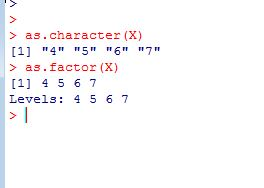
\includegraphics[width=0.7\linewidth]{images/typeconversion} 
 \end{figure}
    
 
 
 
 %==============================================================================================%
 
 % % SLIDE 1 - COVER SLIDE
 \begin{figure}
 \centering
 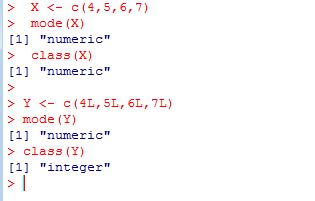
\includegraphics[width=0.7\linewidth]{images/numerictypes}    
 \end{figure}
    
 %==============================================================================================%
 
 \frametitle{1.4 Commenting}
 For the sake of readability, it is good practice to comment code. The \# character at the
 beginning of a line signifies a comment, which is not executed. Lines of hashtags can be used
 to identify the beginning and end of code segments
 
 \begin{semiverbatim}
 # This is a comment
 #####################
 # Start of Segment 1
 #####################
 \end{semiverbatim}
 \end{framed}
 
 %==============================================================================================%
 
 \frametitle{1.5 Defining and Naming Variables}
 
*  A convention is to use define a variable name with a capital letter (R is case sensitive). 
*  This
 reduces the chance of overwriting in-build R functions, which are usually written in lowercase
 letters. 
*  Commonly used variable names such as x,y and z (in lower case letters) are not “reserved”.

 
 \begin{semiverbatim}
 camelCase
 
 variableName
 
 AlsoCamelCase
 \end{semiverbatim}
 
 %==============================================================================================%
 
 % % SLIDE 1 - COVER SLIDE
 \begin{figure}
 \centering
 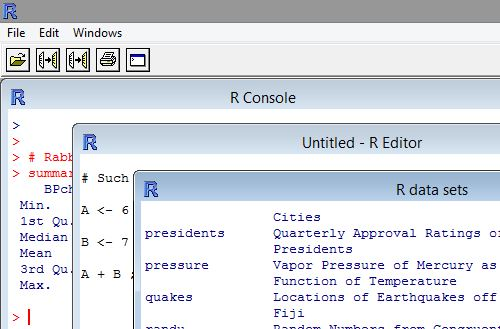
\includegraphics[width=0.7\linewidth]{images/Rmultiplewindows}
 \end{figure}
 
    
 %==============================================================================================%
 
 % % SLIDE 1 - COVER SLIDE
 \begin{figure}
 \centering
 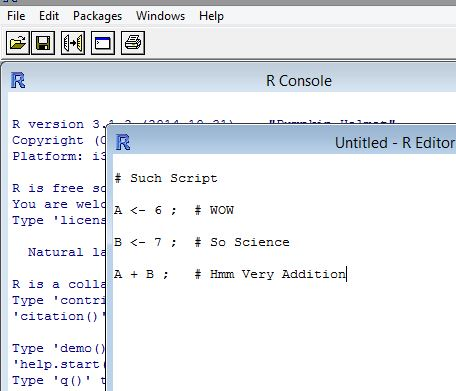
\includegraphics[width=0.7\linewidth]{images/Rscript}         
 \end{figure}
    
 %==============================================================================================%
 
 
 \frametitle{1.6 Help Functions}
 
*  Help files for R functions are accessed by preceding the name of the function with ? (e.g. ?sort
 ). 
 
*  Alternatively you can use the command \texttt{help()} (e.g. help(sqrt) )

 
 
 %==============================================================================================%
 
 
 \frametitle{1.6 Help Functions}
 
*  A HTML document appears on screen with information on the function typed in. 
*  As well
 as the list of arguments that the particular function accepts, and how to specify them, there is
 example code at the bottom of the file. 
*  These code segments are often invaluable in learning
 how to master the function.

 
 
 
 
 
 %==============================================================================================%
 
 % % SLIDE 1 - COVER SLIDE
 \begin{figure}
 \centering
 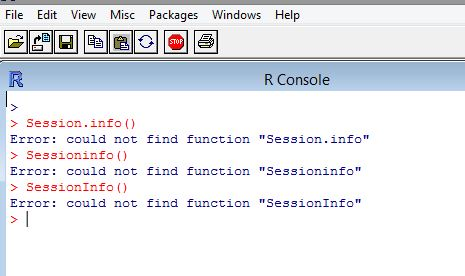
\includegraphics[width=0.7\linewidth]{images/Rapropos1}       
 \end{figure}
    
 %==============================================================================================%
 
 % % SLIDE 1 - COVER SLIDE
 \begin{figure}
 \centering
 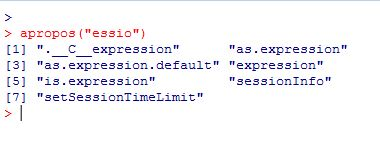
\includegraphics[width=0.7\linewidth]{images/Rapropos2}       
 \end{figure}
    
 %==============================================================================================%
 
 
 
 \frametitle{1.7 The help.start() command}
 As mentioned by the text on the main console, the \texttt{help.start()} command can be usd to
 access detailed help documentation that comes as part of the installation.
 
 %==============================================================================================%
 
 1.9 Basic R Editor
 R has an inbuilt script editor. We will use it for this class, but there are plenty of top quality
 Integrated Development Environments out there. (Read up about RStudio for example).
 For a while, we will use the in-built script editor. Although it is advisable to start using Rstudio or something similar.
 
 
 %==============================================================================================%
 
 
 
 To start a new script, or open an existing script simply go to File and click the appropriate
 options. A new dialogue box will appear. You can write and edit code using this editor.
 To pass the code for compiling , press the run line or selection option (The third icon
 on the menu).
 
 
 %==============================================================================================%
 
 
 Another way to read code is to use the edit() function , which operates directly from the
 command line. To see how the code defining an object X was written (or more importantly,
 could have been written) simply type \texttt{edit(X)}. This command has some useful applications
 that we will see later on.
 
 
 %==============================================================================================%
 
 
 \textbf{Script Files}
 
*  Scripts are saved as \texttt{.R} files. 
*  These scripts can be called directly using the \texttt{source()} command.

 
 %==============================================================================================%
 
 
 %==============================================================================================%
 
 \frametitle{1.11 The summary() command}
 The R command summary() is a generic function used to produce result “summaries” of the
 results of various objects, from simple vectors to the output of complex model fitting functions.
 The function invokes particular methods which depend on the class of the first argument.
 > summary(Nile)
 Min. 1st Qu. Median Mean 3rd Qu. Max.
 456.0 798.5 893.5 919.4 1032.0 1370.0
 
 %==============================================================================================%
 
 > summary(Indometh)
 Subject time conc
 1:11 Min. :0.250 Min. :0.0500
 4:11 1st Qu.:0.750 1st Qu.:0.1100
 2:11 Median :2.000 Median :0.3400
 5:11 Mean :2.886 Mean :0.5918
 6:11 3rd Qu.:5.000 3rd Qu.:0.8325
 3:11 Max. :8.000 Max. :2.7200
 

 %==============================================================================================%
 
 \frametitle{1.13 Coming Unstuck}
 
 
* If you are having trouble with a piece of code that is currently compiling , all you have to do is press ESC, just like many other computing environments.

 
 %==============================================================================================%
 
 \frametitle{1.14 Quitting the R environment}
 As the front page text indicates, all you have to do to quite the workspace is to type in \texttt{q()}.
 You will then be prompted to save your work.
 
 %==============================================================================================%
 
 \frametitle{1.15 Data Objects}
 As mentioned previously, R saves data as \textbf{objects}. Examples of data objects are
 
*  Vectors
*  Lists
*  Dataframes
*  Matrices

 The simple objects we have created previously are simply single element vectors.
 
 %==============================================================================================%
 
 \frametitle{1.16 Listing all items in a workspace}
 To list all items in an R environment, we use the \texttt{ls()} function. This provides a list of all data
 objects accessible. Another useful command is \texttt{objects()}.
 
 \begin{semiverbatim}
 > ls()
 [1] "a" "A" "authors" "b" "books"
 [6] "C" "D" "ex1" "Gerb" "Lst"
 [11] "m" "m1" "op" "presidents" "r"
 [16] "showSmooth" "sm" "sm.3RS" "sm2" "sm3"
 [21] "Trig" "Vec1" "x" "X" "x.at"
 [26] "x1" "x2" "x3R" "y" "Y"
 [31] "y.at"
 \end{semiverbatim}
 \end{framed}
 
 %==============================================================================================%
 
 \frametitle{1.17 Removing items}
 
*  Sometimes it is desirable to save a subset of your workspace instead of the entire workspace.
*  One option is to use the \texttt{rm()} function to remove unwanted objects right before exiting your R
 session; another possibility is to use the \texttt{save()} function.

 
 %==============================================================================================%
 
 \frametitle{1.18 Saving and Loading R Data Objects}
 In situations where a good deal of processing must be used on a raw dataset in order to prepare
 it for analysis, it may be prudent to save the R objects you create in their internal binary form.
 One attractive feature of this scheme is that the objects created can be read by R programs
 running on different computer architectures than the one on which they were created, making it
 very easy to move your data between different computers. Each time an R session is completed,
 you are prompted to save the workspace image, which is a binary file called .RData in the
 working directory.
 
 %==============================================================================================%
 
 Whenever R encounters such a file in the working directory at the beginning of a session,
 it automatically loads it making all your saved objects available again. So one method for
 
 saving your work is to always save your workspace image at the end of an R session. If you
 would like to save your workspace image at some other time during your R session, you can use
 the save.image() function, which, when called with no arguments, will also save the current
 workspace to a file called .RData in the working directory.
 
 
 
 %==============================================================================================%
 
 %2 Introduction to R (Continued)
 \frametitle{2.1 Three particularly useful commands}
 
 
*  \texttt{help()}
*  \texttt{summary()}
*  \texttt{help.start()}

 
 
 %==============================================================================================%
 
 \frametitle{2.2 Changing GUI options}
 
*  We can change the GUI options using the GUI preferences option on the Edit menu.
*   (Important
 when teaching R) 
*  A demonstration will be done in class.

 
 
 %==============================================================================================%
 
 \frametitle{2.3 Colours}
 
*  R supported a massive number of colours.
*  Type in colours() (or colors()) to see what colours
 are supported.

 
 %==============================================================================================%
 
 \frametitle{2.4 Use of the Semi-Colon Operator}
 
*  The semi-colon operator at the end of each line of code is not necessary in general, but using it
 overcomes errors due to copying and pasting from document soft copies. 
*  It is also useful for compacting multiple short statements onto a single line.
*  In other programming
 languages, such as Octave, using the semicolon in this way has a distinct purpose.

 
 %==============================================================================================%
 
 \frametitle{2.5 The apropos() Function}
 This function is very useful for determining what functions are available for a particular topic,
 although the process requires a great deal of trial and error. Suppose we are looking for a
 command to compute the correlation coefficient. We would use a very short string (e.g. cor)
 that would plausibly be part of useful function names.
 
 
 %==============================================================================================%
 
 \frametitle{2.6 History}
 
*  The command \texttt{history()} is used to obtain the last 25 commands used by <tt>R</tt>.
*  25 is the default number, you can specify another number.

 
 \begin{semiverbatim}
 history(100)
 \end{semiverbatim}
 \end{framed}
 
 
 %==============================================================================================%
 
 % % SLIDE 1 - COVER SLIDE
 \begin{figure}
 \centering
 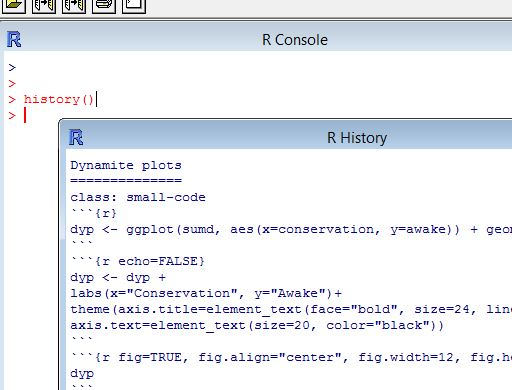
\includegraphics[width=0.7\linewidth]{images/Rhistory}        
 \end{figure}
    
 %==============================================================================================%
 
 \frametitle{2.7 The \texttt{sessionInfo()} Function}
 To get a description of the version of R and its attached packages used in the current session,
 we can use the \texttt{sessionInfo()} function
 
 
 %==============================================================================================%
 
 \frametitle{2.8 Time and date functions}
 The commands Sys.time() and Sys.Date() returns the system’s idea of the current date
 with and without time. We can perform some simple algebraic calculations to compute time
 differences (i.e. to find out how long some code took to compile.
 
 
 %==============================================================================================%
 
 \frametitle{System Time}
 
 \begin{semiverbatim}
 > X1=Sys.time()
 > #Wait a few seconds
 >
 > X2=Sys.time()
 > X2-X1 Time difference of 8.439614 secs
 >
 > Sys.Date() [1] "2012-09-01"
 \end{semiverbatim}
 \end{framed}
 
 %==============================================================================================%
 
 \frametitle{2.9 Logical States}
 
*  Logical states TRUE and FALSE are simply specified as such, all in capital letters. 
*  The
 shortcuts T and F are also recognized

 
 %==============================================================================================%
 
 
 
 2.10 Missing Data
 In some cases the entire contents of a vector may not be known. For example, missing data
 from a particular data set. A place can be reserved for this by assigning it the special value
 NA.
 NA is a logical constant of length 1 which contains a missing value indicator. NA stands
 for Not Available.
 
 
 %==============================================================================================%
 
 
 \frametitle{2.11 Files in the Working Directory}
 It is possibel to call an R script from the working directory, using the \texttt{source()} function.
 
 \begin{semiverbatim}
 source("myfunctions.r")
 source("mydata.r")
 \end{semiverbatim}
 \end{framed}
 We can also send code put directly to a file in the working directory, using the sink()
 command. The first time the command is used, the name of the created file is specified.
 Subsequent commands print output directly to this file, until the command is used again to
 cease the operation.
 
 %==============================================================================================%
 
 
 \begin{semiverbatim}
 > sink("IrisSum.txt")
 > summary(iris)
 > sink()
 >
 \end{semiverbatim}
 \end{framed}
 
 
 %==============================================================================================%
 
 
 \frametitle{3.3 Structure of a Data Object}
 
 The structure, class and storage mode of an object can be determined using the following
 commands. Try out a few.
 
*   \texttt{str()}
*   \texttt{class()}
*   \texttt{mode()}

 
 
 
 %==============================================================================================%
 
 
 \begin{semiverbatim}
 > class(Nile)
 [1] "ts"
 > mode(Nile)
 [1] "numeric"
 >
 
 \end{semiverbatim}
 \end{framed}
 
 
 %==============================================================================================%
 
 \begin{semiverbatim}
 > a
 [1] 6
 > mode(a)
 [1] "numeric"
 > class(a)
 [1] "numeric"
 > str(a)
 num 6
 >
 > class(iris)
 [1] "data.frame"
 > mode(iris)
 [1] "list"
 \end{semiverbatim}
 
 
 %==============================================================================================%
 
 
 \Huge
 \[\mbox{ Section 4 : Packages } \]
 
 
 \frametitle{Packages}
 
 
*  A Package in <tt>R</tt> is a file containing a collection of objects which have some common purpose.
*  Packages enhance the capabilties and scope for research in a certain field. 
*  For example, the
 package MASS contains objects associated with the Venables and Ripleys ``\textit{Modern Applied
 Statistics with S}”. 

 
 
 %=================================================================== %
 
 
 
 \begin{figure}
 \centering
 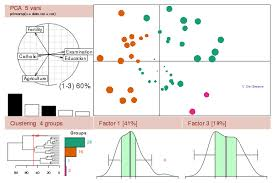
\includegraphics[width=0.97\linewidth]{CRAN}
 \caption{Comprehensive R Archive Network}
 
 \end{figure}
 
 
 
 
 
 %=================================================================== %
 
 \frametitle{R Packages}
 
 
*  ``10 R packages I wish I knew about earlier" - Drew Conway (Yhat.com, February 2013)
 \bigskip*  ``The HadleyVerse" - Hadley Wickham
 
 
*   ggplot2, dplyr, reshape, lubridate, stringr
 
*   With Romain Francois, Dianne Cook and Garret Grolemund.

 \bigskip
*  Dr Brendan Haplin (UL): lme4 ,TraMineR, Gelman's arm, MASS, foreign. 
 \bigskip
*  Shiny - Web Applications with <tt>R</tt>

 
 %=================================================================== %
 
 \frametitle{R Packages}
 
 
 
 
 Some examples of packages are Actuar, written for actuarial science, and
 QRMlib, which complements the Quantitative Risk Management The command library()
 lists all the available packages. 
 
 To load a particular package, for example MASS, we would
 write
 library(MASS)
 
 
 %=================================================================== %
 
 
 \frametitle{Packages}
 
*  The CRAN package repository features 6107 available packages. 
*  Packages contain
 various functions and data sets for numerous purposes, e.g.
 \textbf{\textit{ggplot2}} package, \textbf{\textit{AER}} package, \textbf{\textit{survival}} package, etc.
*  Some packages are part of the basic installation. Others can be
 downloaded from CRAN.
*  To access all of the functions and data sets in a particular package,
 it must be loaded into the workspace. 
*  For example, to load the
 \textbf{\textit{ggplot2}} package:

 
 \begin{semiverbatim}
 install.packages(ggplot2)
 library(ggplot2)
 \end{semiverbatim}
 \end{framed}
 
 %==============================================================================================%
 
 \frametitle{4.2 Using and Installing packages}
 
*  Many packages come with R. To use them in an R session, you need to load the package, as
 previously demonstrated.
*  Some packages are not automatically installed when you install R but they need to be downloaded
 and installed individually. 
*  We must first install them using the install.packages()
 function, which typically downloads the package from CRAN and installs it for use. (follow the
 instructions as indicated).

 
 %==============================================================================================%
 
 
 \begin{semiverbatim}
 install.packages("ggplot2")
 install.packages("qcc")
 install.packages("sqldf")
 install.packages("RMongo")
 install.packages("randomforest")
 \end{semiverbatim}
 \end{framed}
 
 
 %==============================================================================================%
 
 \frametitle{4.2.1 Version of R}
 Many packages will require you to have the most recent version of R and also other packages.
 It is a good idea to update regularly.
 
 %==============================================================================================%
 
 5 Data Creation, Data Entry, Data Import and Export
 
 %==============================================================================================%
 
 \frametitle{5.1 The \texttt{c()} command}
 To create a simple data set, known as a vector, we use the c() command to create the vector.
 
 \begin{semiverbatim}
 > Y=c(1,2,4,8,16 ) #create a data vector with specified elements
 > Y
 [1] 1 2 4 8 16
 
 \end{semiverbatim}
 \end{framed}
 
 
 %==============================================================================================%
 
 \frametitle{Vectors}
 
 \begin{semiverbatim}
 ### Vector of Numeric Values
 Numvec = c(10,13,15,19,25);
 ## Vector of Character Values
 Charvec = c("LouLou","Oscar","Rasher");
 
 ## Vector of Logical Values
 Charvec = c(TRUE,TRUE,FALSE,TRUE);
 \end{semiverbatim}
 \end{framed}
 
 %==============================================================================================%
 
 \frametitle{Vectors}
 Vectors can be bound together either by row or by column.
 
 \begin{semiverbatim}
 > X=1:3; Y=4:6
 > cbind(X,Y)
 X Y
 [1,] 1 4
 [2,] 2 5
 [3,] 3 6
 >
 > rbind(X,Y)
 [,1] [,2] [,3]
 X 1 2 3
 Y 4 5 6
 \end{semiverbatim}
 \end{framed}
 
 %==============================================================================================%
 
 \frametitle{5.2 The scan() command}
 
* The \texttt{scan()} function is a useful method of inputting data quickly. 
*  You can use to quickly copy
 and paste values into the <tt>R</tt> environment. It is best used in the manner as described in the
 following example. 
*  Create a variable ”X” and use the \texttt{scan()} function to populate it with
 values. 
*  Type in a value, and then press return. Once you have entered all the values, press
 return again to return to normal operation.

 
 %==============================================================================================%
 
 \begin{semiverbatim}
 > X=scan()
 1: 4
 2: 5
 3: 5
 4: 6
 5:
 Read 4 items
 \end{semiverbatim}
 Remark: Try the \texttt{edit()} command on object X.
 
 %==============================================================================================%
 
 5.2.1 Characters with the scan() command
 The scan() command can also be used forinputting character data.
 > Y=scan(what=" ")
 1: LouLou
 2: Oscar
 3: Rasher
 4:
 Read 3 items
 > Y
 [1] "LouLou" "Oscar" "Rasher"
 
 %==============================================================================================%
 
 5.3 Using the data editor
 
 
 %==============================================================================================%
 
 5.4 Spreadsheet Interface
 R provides a spreadsheet interface for editing the values of existing data sets. We use the
 command \texttt{data.entry()}, and name of the data object as the argument. (Also try out the
 fix() command)
 
 \begin{semiverbatim}
 > data.entry(X) # Edit the data set and exit interface
 > X
 \end{semiverbatim}
 \end{framed}
 
 
 
 
 
 
 
\end{document}
